\chapter{Exploration of atomistic predictions}
\label{chapter2}

Atomic interactions are the foundation on which many ML models---especially interatomic potential models---are built.
Accuracy is well-defined in quantum chemical methods via systematic convergence and comparison to experimental data, but wavefunction-based approaches are computationally expensive and are limited to system sizes of only a handful of atoms.
Measuring predictive accuracy is difficult when approximating the results of first principles computations for systems that exceed the size limitations of QM approaches.
This raises a vital question to the efficacy of ML models: how do we assess the reliability of atomistic neural network potential models for systems that exceed the size limitations of QM computations?

The scalability of NNP models stems from partitioning molecules into atomic components, characterized by their local chemical environment.
However, this introduces new challenges in generalization and transferability and, therefore, model reliability when exposed to new atomic interactions during inference.
This chapter serves as an assessment of the reliability of model predictions of molecular enery and atomistic energy contributions in ANAKIN-ME neural network potential models.
Section \ref{sec:ANI_predictions} contains a detailed look at the predictions of ANI neural networks from atomistic features to global properties and the measure of uncertainty used to determine the trustworthiness of a prediction.
The following section, \ref{sec:uncertainty_atomic_energies}, details the search for an improved metric of reliability in atomistic predictions.

\section{ANAKIN-ME predictions}
\label{sec:ANI_predictions}

The ANI methodology provides a framework for atom-wise decomposition of molecular energies by using the atomic environment vector (AEV) representation to encode localized chemical interactions.
A decomposition approach allows for efficient, scalable predictions of energy for systems larger than the training data represents.
This is advantageous for simulating large systems, due to the size limitations of \textit{ab initio} computations.
The driving idea behind the AEV representation is that all atomic interactions within a system can be characterized by the localized environment. 
This neglects long-range interactions such as van der Waals forces and electrostatics, which are undoubtedly important for some systems, but has little influence on the predictive accuracy of single-point calculations of small organic molecules.
Corrective approaches to long-range interactions have been explored, such as ANI-MBIS-q \cite{ml_mm_santi_y_jonny2}, which considers long-range electrostatics using a separate, parallel network to predict partial charges.
For small, charge-neutral molecules, localized interactions encoded in the AEV have been shown to capture the relationship between molecular energy and atomic species and their positions \cite{ani-1, ani-1x, ani-2x}.

Though some partitioning schemes exist in quantum theory, such as Bader's Atoms in Molecules \cite{bader_aim}, there is no general consensus for decomposing the energy of a molecular system into a sum of atomic contributions.
The energy decomposition approach taken by ANI is a learned relationship decided by the individual atomic neural networks during training, explained in greater detail in Subsection \ref{subsec:total_E_sum_AEs}.
The uncertainty measure of predicted energies, referred to as the QBC, is defined in Subsection \ref{subsec:ANI_uncertainty}, followed by a case study in Subsection \ref{subsec:flaws_in_qbc} of the reliability of the QBC as a measure of empirical uncertainty in ANI predictions.

\subsection{Molecular energy as a sum of atomic contributions}
\label{subsec:total_E_sum_AEs}

The predicted molecular energy for a molecule input to an ANI model is computed as a sum of atomic contributions, given in Eqn. \ref{eq:total_E_sum_AEs}, where $E_{\text{Total}}$ is the molecular energy prediction and $\varepsilon_i$ is the atomic energy contribution for atom $i$.

\begin{equation}
    E_{\text{Total}} = \sum_{i}^{\text{atoms}} \varepsilon_i
    \label{eq:total_E_sum_AEs}
\end{equation}

To visualize atomic energy predictions, a small testing subset was created using the first conformer of each molecular formula in the ANI-1x training dataset.
This testing set, referred to as 1x-test ($N=$ 3,114), is used to explore some trends in predicted atomic energies for the carbon, hydrogen, nitrogen, and oxygen atom types across an ensemble of eight models.
Testing on this subset gives insight on the performance of ANI models for well-characterized systems, as this was the data used in training the model.
The ANI-1x and 2x potential models were trained using self-atomic energies (SAEs), where the predicted atomic energy values form a distribution centered at zero. 
This means that, by definition, each atom has either no net contribution to the molecular energy, or contributes an energy deviation that is relative to the baseline for that atom type.
The atomic energy contributions predicted by the ANI-2x model for C, H, N, and O atoms across the 1x-first test set are given in Figure \ref{fig:2x_ae_per_model}.

\begin{figure}[!h]
    \centering
    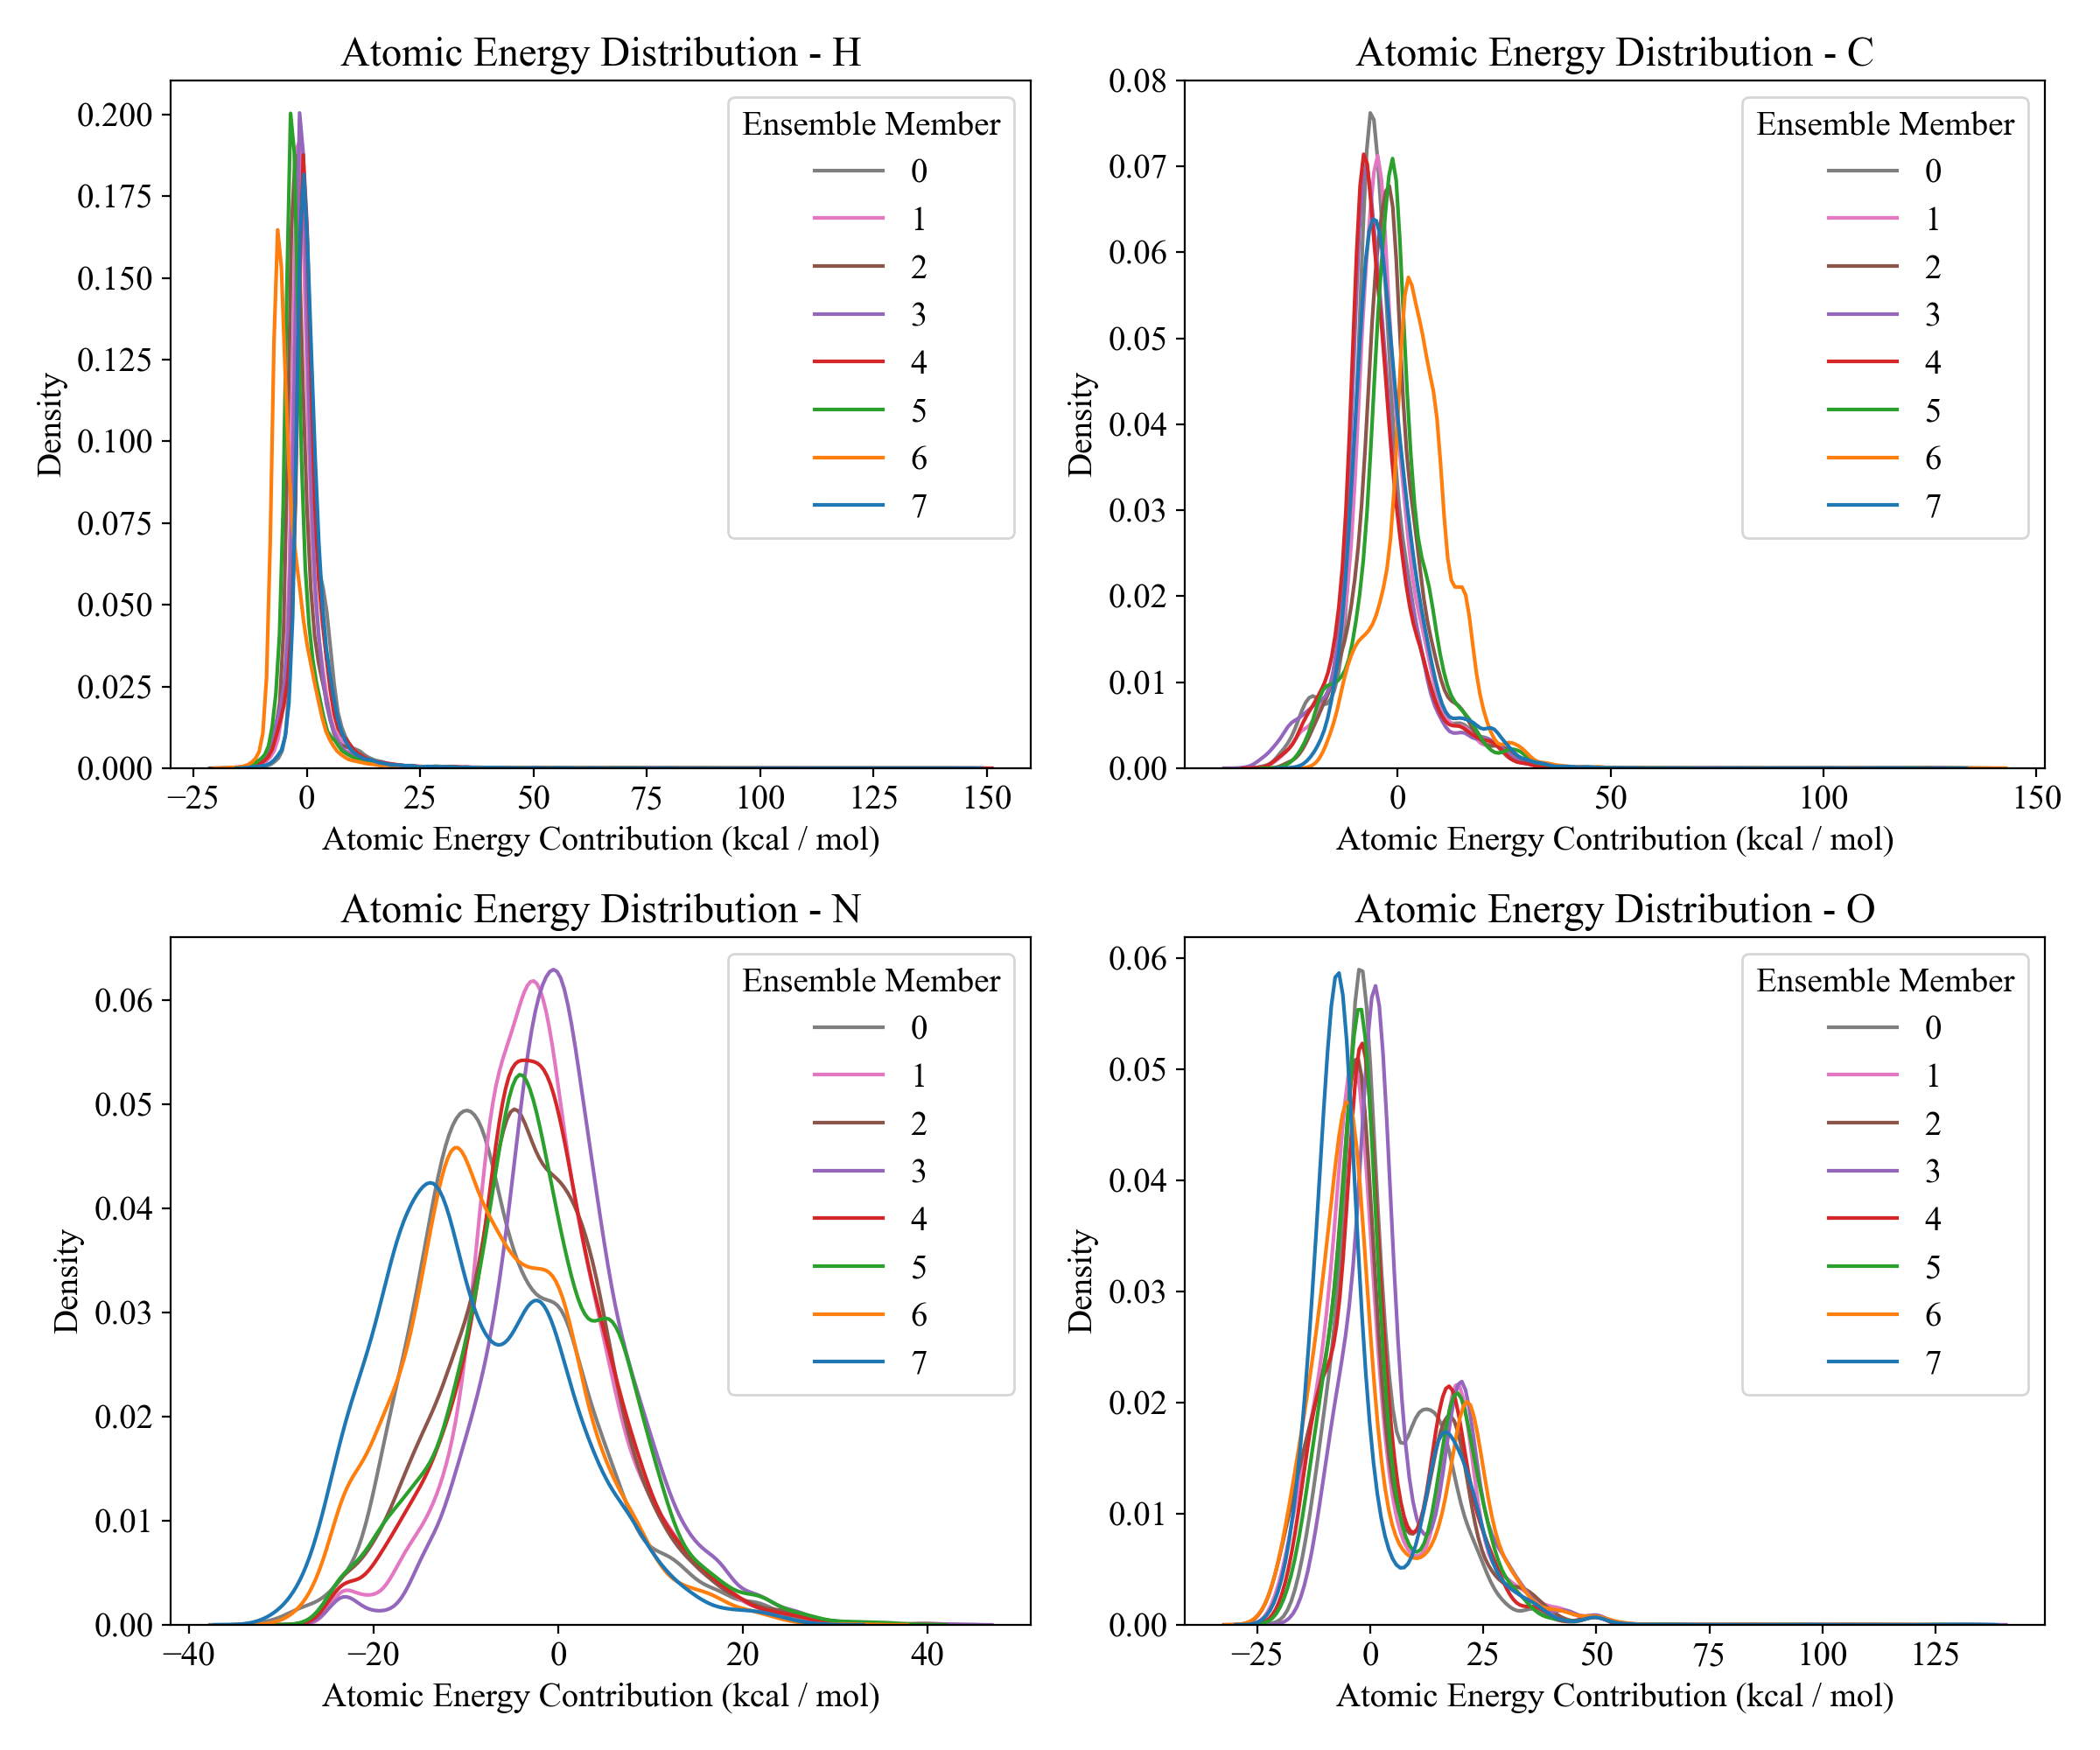
\includegraphics[width=1\linewidth]{Images/2x_outputs/2x_1x-first_ae-per-model.png}
    \caption[Atomic energies predicted by ANI-2x]{Per-model distribution of atomic energy contributions by atom type for the ANI-2x potential. Values shown in kcal/mol for HCNO atom types on the 1x-first subset.}
    \label{fig:2x_ae_per_model}
\end{figure}

Shifting atomic energies with SAEs causes the model to learn relative energy contributions rather than absolute values. 
Refined ANI models, such as ANI-2xr, are trained with slightly different hyperparameters.
The largest change between ANI-2x and 2xr is the removal of biases from neuron outputs; Eqn. \ref{eq:nn_eqn} shows the method for computing the weighted-sum output of each neuron ($y$) from the input ($x_i$) multiplied by its weight ($w_i$).
Traditionally, artificial neural networks use biases to output some value, even when the weighted sum of input values is close or equal to zero.
For interatomic potentials, if we pass a single atom with no neighbors through a network, we would expect to get exactly the energy of that atom in space with no other interacting particles.
By removing the biases from the species-specific networks, we can achieve this goal and add a bit more physicality to the behavior of the neural network outputs.
To replace the biases, we add a final shift to the output: the EnergyShifter.
This is a protocol within TorchANI which adds the ground state atomic energy (GSAE) to each atom, shifting the output values of the NNs toward physically meaningful values.
Ground state atomic energies are calculated at the level of theory used in producing training data from a neutrally charged atom isolated in space with the proper spin multiplicity (ensuring a ground-state electronic configuration).
Thus, the total energy prediction in ANI-2xr networks are computed as shown in Equation \ref{eq:total_E_GSAEs}.

\begin{equation}
    E_{\text{Total}} = \sum_{i}^{\text{atoms}} \varepsilon_i + \text{GSAE}_i
    \label{eq:total_E_GSAEs}
\end{equation}

Here, the total energy is a sum of atomic contributions as in Eqn. \ref{eq:total_E_sum_AEs}, and $\text{GSAE}_i$ is the ground state atomic energy for atom $i$, which shift the network outputs toward more physically meaningful values.
The ground state atomic energies for each atom in the ANI networks are given in \ref{appendix:GSAEs}.
In addition to the removal of biases and the replacement of self-atomic energies with GSAEs, ANI-2xr is trained with the addition of a simple, analytical xTB repulsion term \cite{xtb_repulsion}.
The inclusion of repulsion to the potential introduces more physical behavior in regions of the potential energy surface that are difficult to sample, namely when two atoms get very close together.
Equation \ref{eq:repulsion} shows the form of this repulsion term for two atoms, where $a$ and $b$ (with atomic numbers $A$ and $B$, respectively) separated by a distance $r_{ab}$. 
The parameters $Y_A$ and $Y_B$ define the magnitude of the repulsive term for their respective elements, $\alpha_{A}$ and $\alpha_{B}$ are element-specific parameters, and $k_{AB}$ is a small correction for very light elements (H, He) and equal to 3/2 in all other cases.

\begin{equation}
\label{eq:repulsion}
    E_{\text{rep}}(r_{ab}) = 
    \sum_{AB}\frac{{Y_{A} Y_{B}}}{r_{ab}}
    \exp \left( -\sqrt{\alpha_{A} \alpha_{B}} {(r_{ab})}^{k_{AB}} \right)
\end{equation}

The ANI-2xr atomic energy distribution for hydrogen, carbon, nitrogen, and oxygen are given in Fig. \ref{fig:2xr_ae_per_model} for an eight-membered ensemble.
Note here that the distributions have slightly different shapes, as well as being shifted far from the zero-centered ANI-2x distributions shown in Figure \ref{fig:2x_ae_per_model}.

\begin{figure}[H]
    \centering
    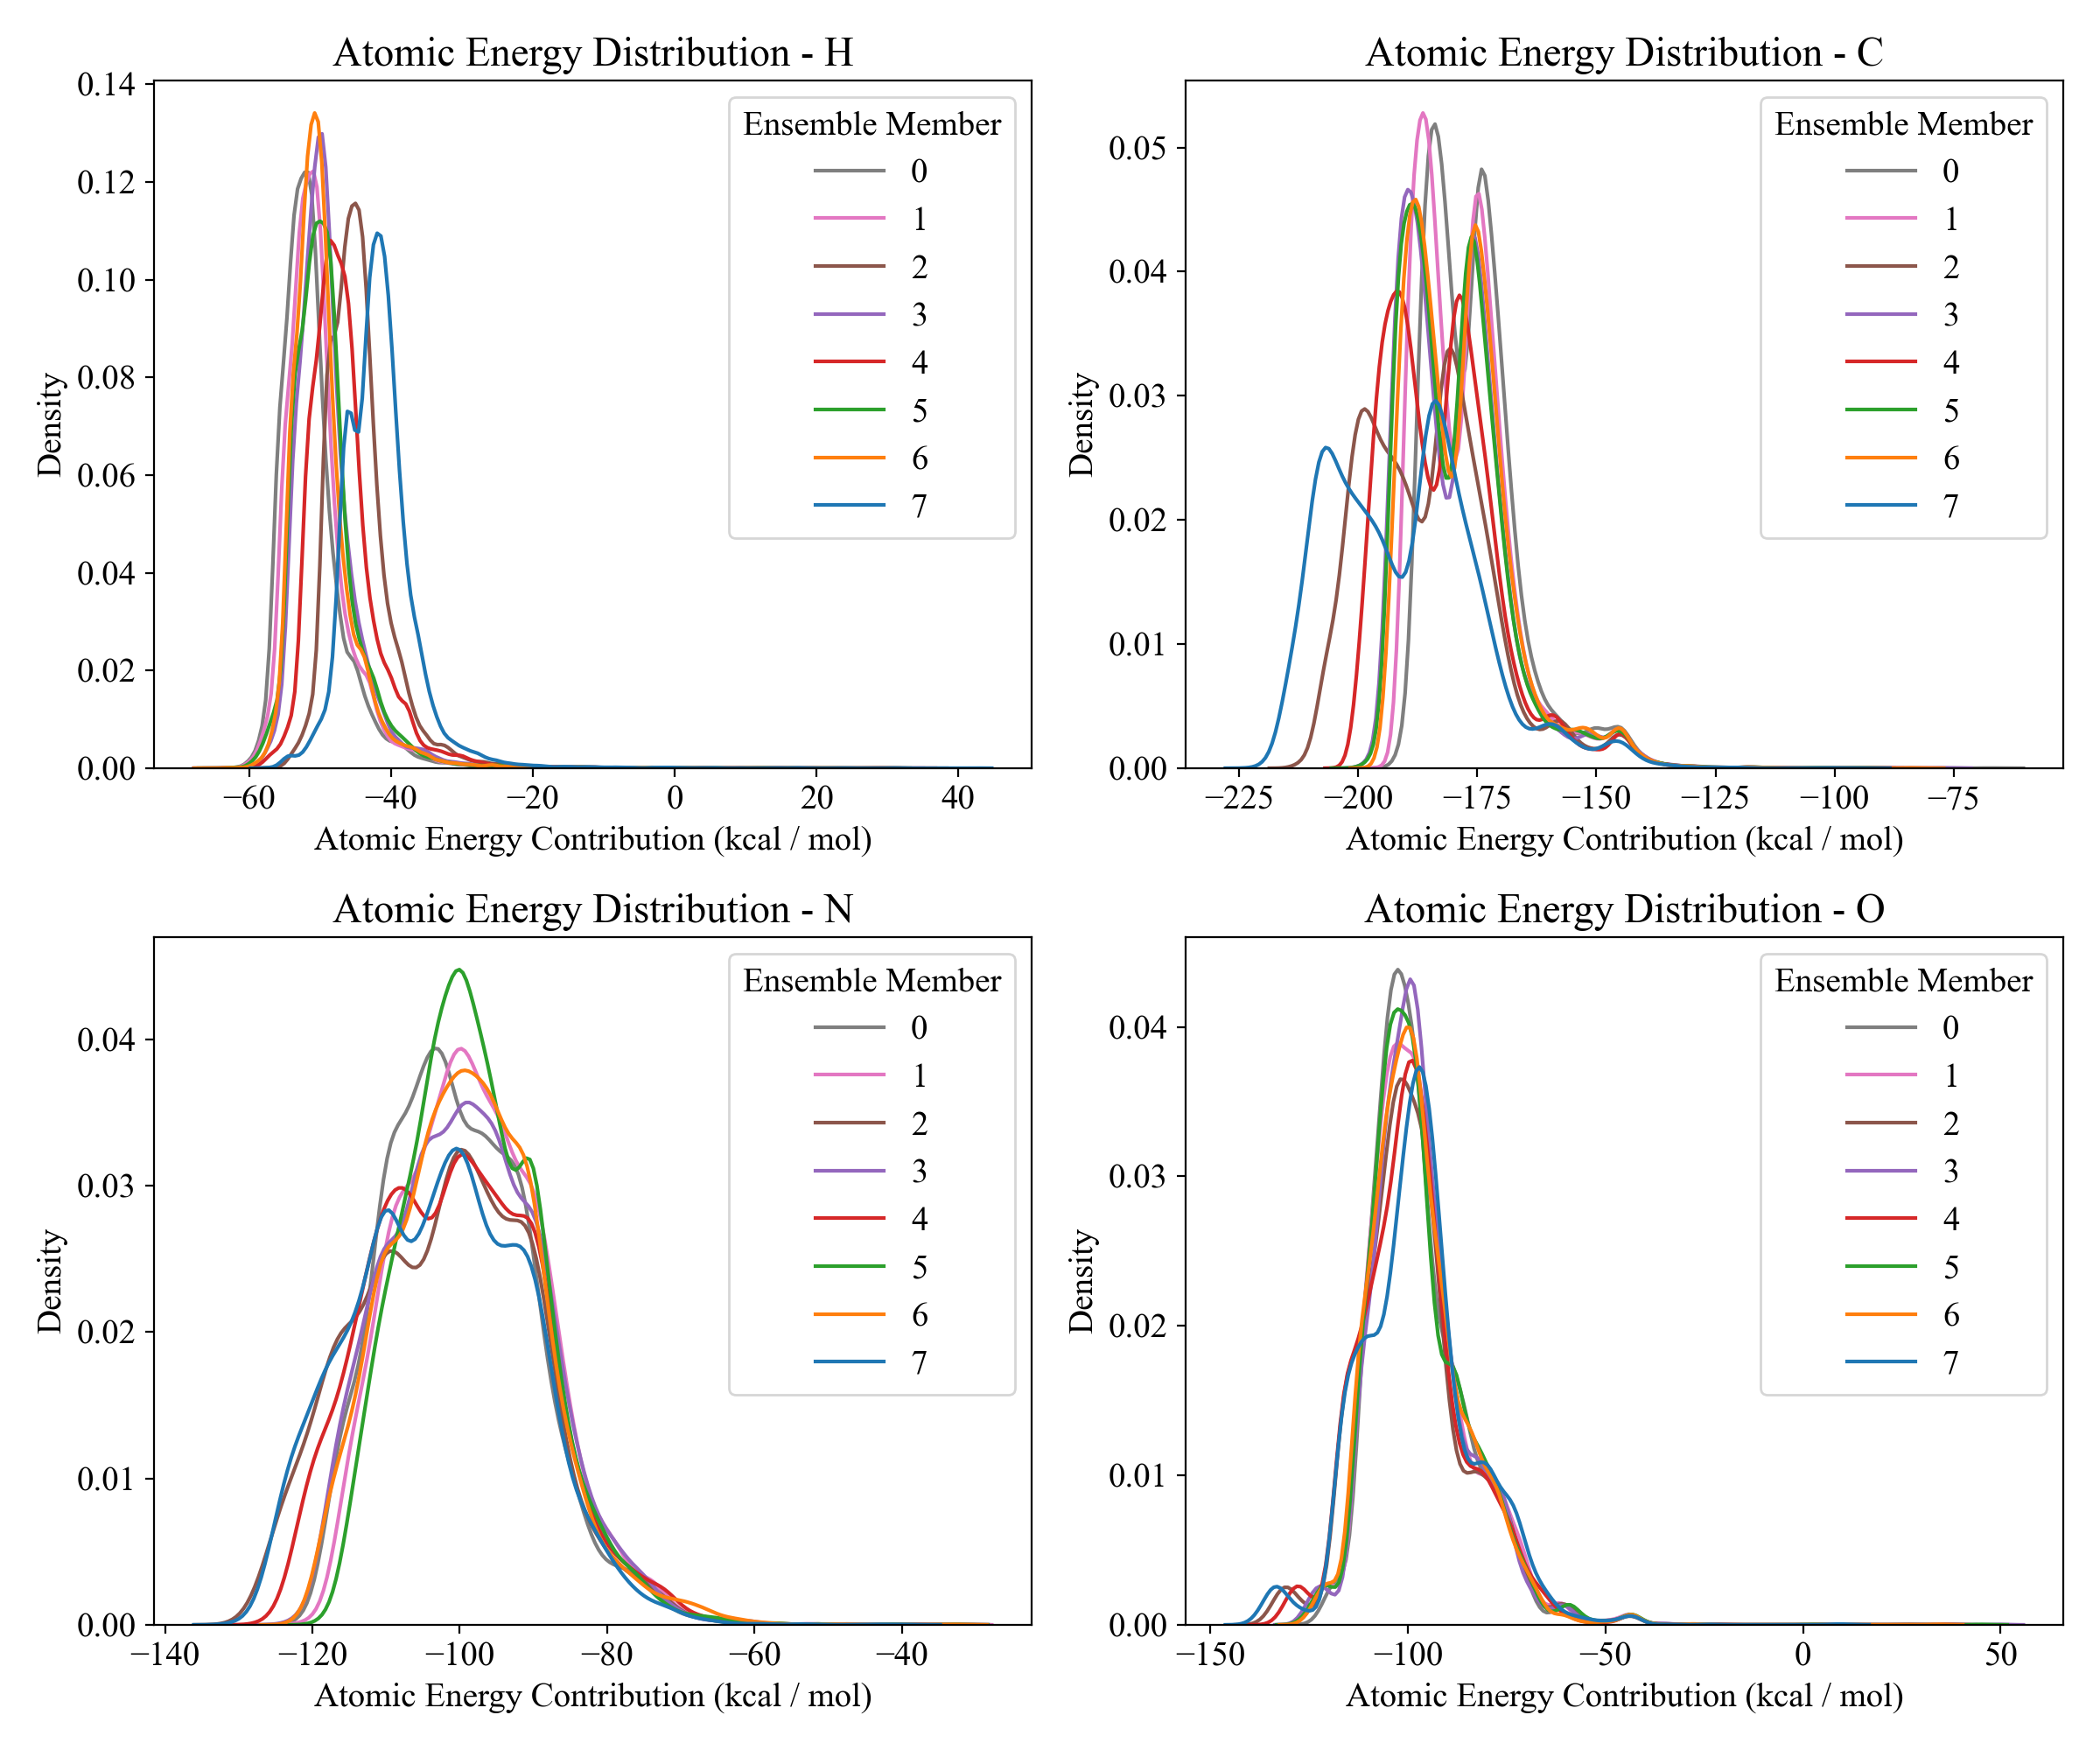
\includegraphics[width=1\linewidth]{Images/2xr_outputs/2xr_1x-first_ae-per-model.png}
    \caption[Atomic energies predicted by ANI-2xr]{Distribution of atomic energy contributions by atom type for the ANI-2xr potential. Values shown in kcal/mol for CHNO atom types on the 1x-first subset.}
    \label{fig:2xr_ae_per_model}
\end{figure}

The difference in the shapes of these distributions is an important aspect of analyzing the predictive uncertainty of ANI neural network potentials.
Due to the differences in hyperparameters used in training, such as the removal of biases, the use of the GELU activation function \cite{gelu} continuous second derivatives improving the smoothness of predicted potential energy surfaces, and the addition of ground state atomic energies and a repulsive term, ANI-2xr will be used to explore trends in uncertainty in predictions by ANI neural networks. 

\subsection{Uncertainty in ANI neural network potentials}
\label{subsec:ANI_uncertainty}

ANI potential models use an ensemble of eight independently models, allowing for the estimation of predictive uncertainty.
Predictive uncertainty has been measured in published models using $\hat{rho}$; the value 0.23 kcal/mol was empirically chosen for sampling structures with high-error energy predictions via query by committee (QBC) in the active learning process \cite{ani-1x}.
The QBC, given in Eqn. \ref{eq:energy_qbc}, can be thought of as a binary classifier: 

\begin{equation}
\rho = \frac{\sigma_{E_{\text{Total}}}}{\sqrt{N_{\text{atoms}}}}
\label{eq:energy_qbc}
\end{equation}

Segue into the atomic energy prediction per atom-type 

\begin{figure}[H]
    \centering
    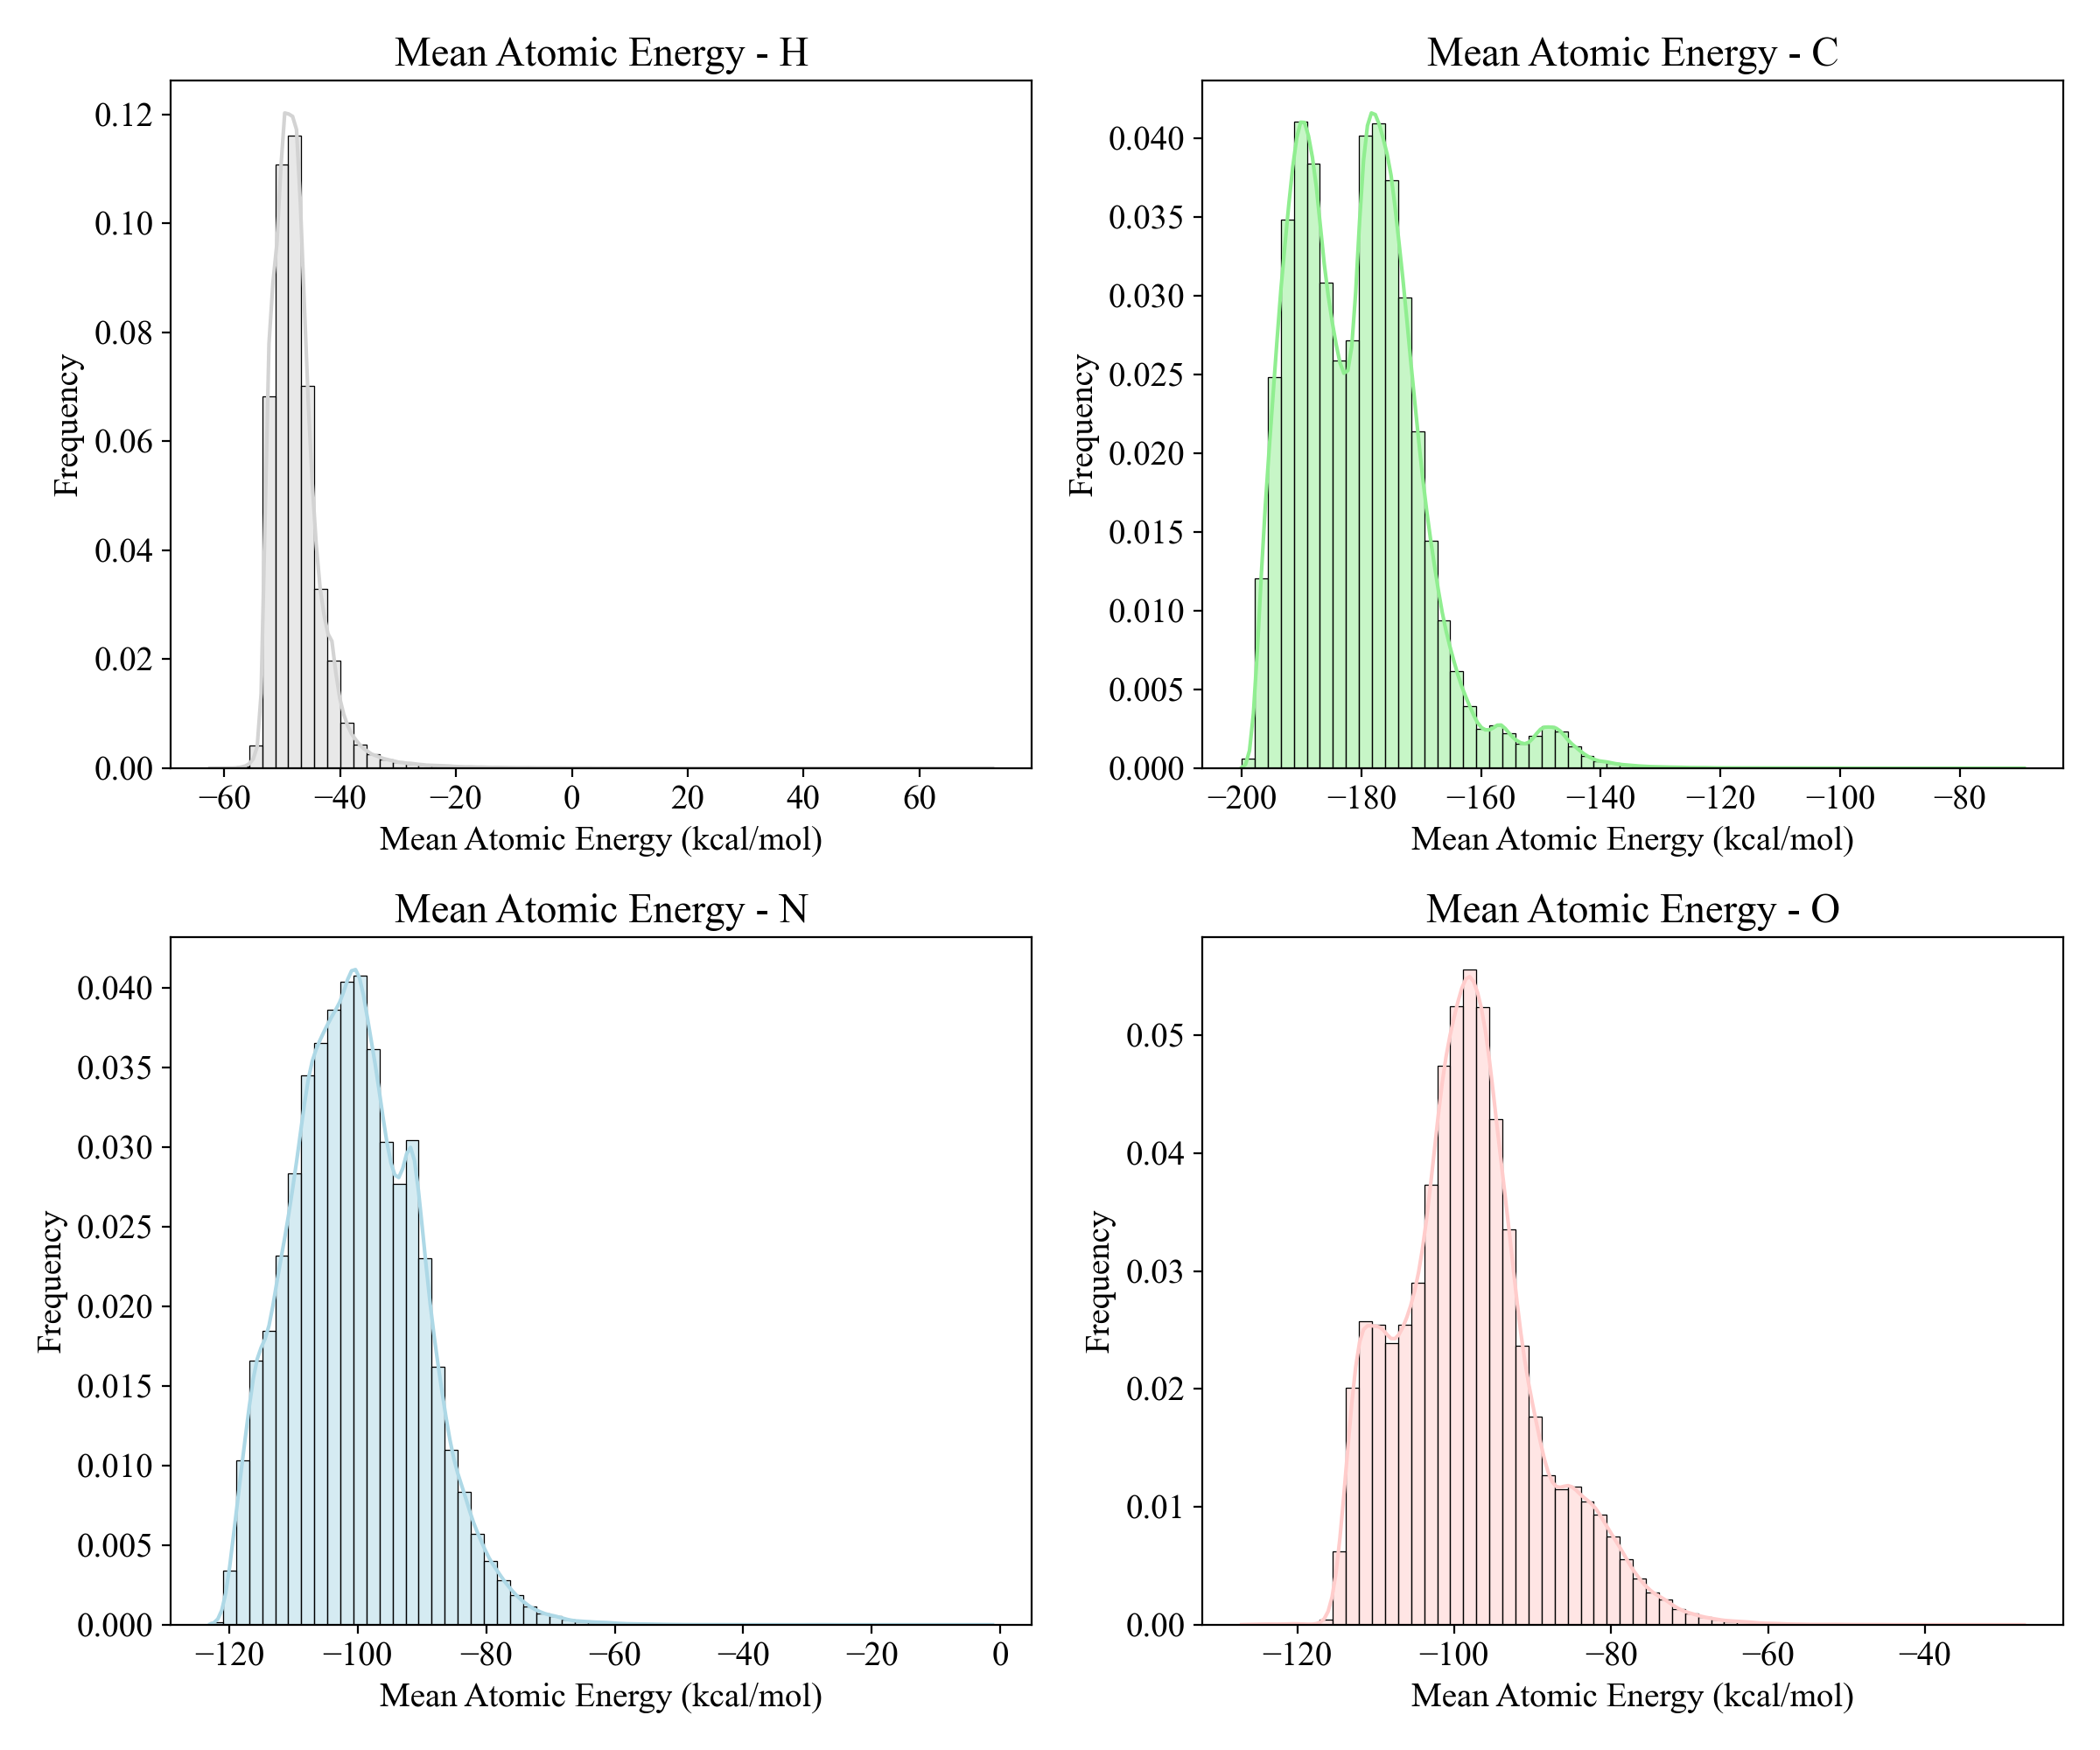
\includegraphics[width=1\linewidth]{Images/2xr_outputs/2xr_comp6v1_mean-ae-per-atomtype.png}
    \caption[Mean atomic energy prediction per-atom with ANI-2xr]{Distribution of predicted mean atomic energies using the ANI-2xr model on the COMP6v1 benchmark set.}
    \label{fig:2xr_comp6v1_mean-ae-per-atomtype}
\end{figure}

\subsection{Exploration of the flaws in measuring uncertainty via predicted total energy}
\label{subsec:flaws_in_qbc}

Make sure to put some words here.
Size dependence of the QBC. \\
Show the example of m-epoxide vs long-epoxide here. Remake those RDKit graphs or consider making vmd figures. 
Also probably want to include some kind of table.

\section{Uncertainty of atomic energy predictions}
\label{sec:uncertainty_atomic_energies}


\begin{figure}[H]
    \centering
    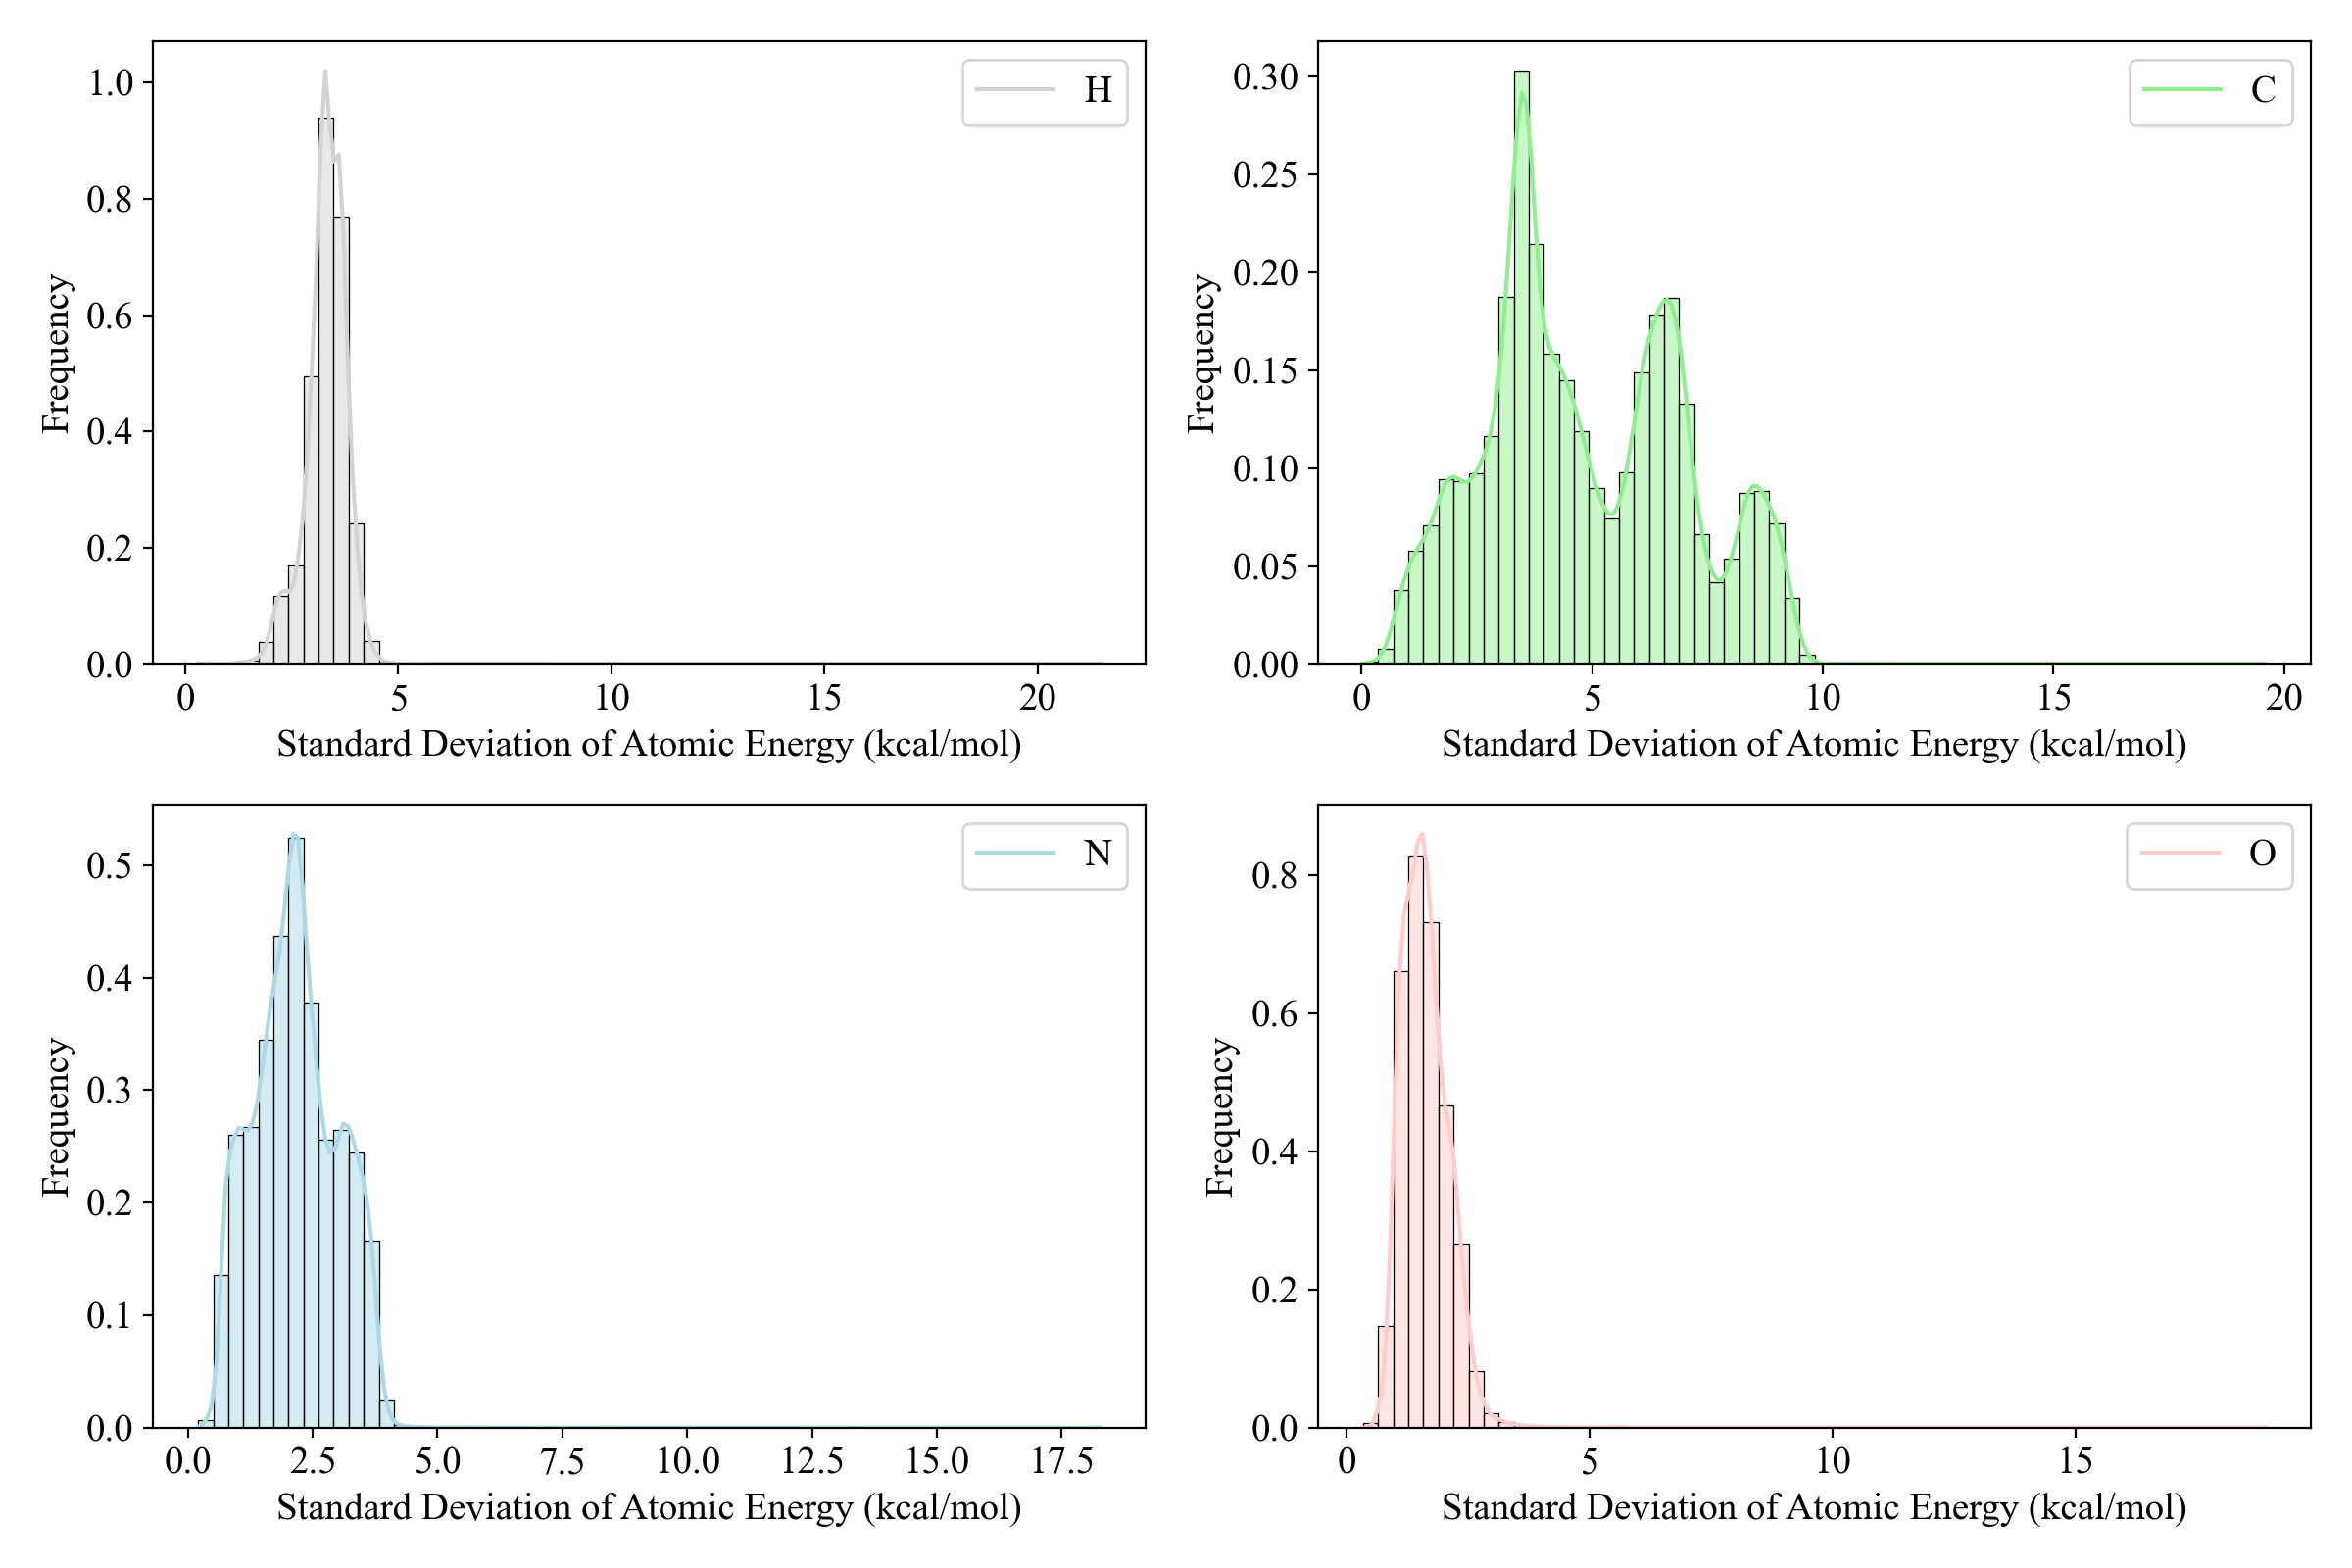
\includegraphics[width=1\linewidth]{Images/2xr_outputs/2xr_comp6v1_stdev-ae-per-atomtype.png}
    \caption[Standard deviation in predicted atomic energy contribution for H, C, N, O atom types]{Distribution of standard deviation in predicted atomic energies using the ANI-2x model on the COMP6v1 benchmark set.}
    \label{fig:2xr_comp6v1_stdev-ae-per-atomtype}
\end{figure}

And also put some words here.
\bigskip




I don't know why this figures is printing weirdly
\\
\begin{flushleft}
\begin{multiFigure}
    \addFigure{0.31}{Images/ch4.png}
    \addFigure{0.68}{Images/ch4_example/ch4_2xr_total-e-qbc.png} \\
    \addFigure{1}{Images/ch4_example/ch4_2xr_stdev-ae.png}
\captionof{figure}[CH\textsubscript{4} atomic energy distribution vs 1x-first]{
(A) Structure of geometry-optimized CH\textsubscript{4}; 
(B) Plot of the distribution of total energy QBC across the 1x-first test set, 
(C) standard deviation in predicted atomic energy for hydrogen (left) and carbon (right); 
the red lines show the standard deviation in CH\textsubscript{4} total energy (B) and atomic energy contributions (C).
}
\label{fig:ch4_stdev_ae}
\end{multiFigure}
\end{flushleft}



% Tables suck, but this helped me align columns and headers separately:
\begin{table}[hbt]
\centering
\caption[CH\textsubscript{4} atomic energy contributions per-model]{
Atomic energy contributions by atom type in a geometry-optimized molecule of CH\textsubscript{4}, with four equivalent hydrogen atoms. 
Additionally, the sum over all atoms, and that sum after passing through the TorchANI EnergyShifter. 
Values obtained from an ensemble of ANI models (ANI2xr); the last column shows the standard deviation of predictions across the ensemble. 
All values are in kcal/mol.
}\label{tbl:ch4_AEs}
    \begin{tabularx}{\textwidth}{%
    >{\raggedleft\arraybackslash}r  % Numeric
    >{\raggedleft\arraybackslash}r  % Numeric
    >{\raggedleft\arraybackslash}r  % Numeric
    >{\raggedleft\arraybackslash}r  % Numeric
    >{\raggedleft\arraybackslash}r  % Numeric
    }  
\hline
Model & Carbon & Hydrogen  & Sum of atomic energies & Molecular energy \\
\hline
Mean prediction & -199.0069 & -55.1013 & -419.4123 & -25413.8125 \\
1 & -219.4329 &  -50.0170 &  -419.5012 &  -25413.9043 \\
2 & -194.7117 &  -56.1991 &  -419.5081 &  -25413.9102 \\
3 & -192.8823 &  -56.6466 &  -419.4689 &  -25413.8691 \\
4 & -201.5683 &  -54.4451 &  -419.3490 &  -25413.7500 \\
5 & -196.5227 &  -55.7060 &  -419.3471 &  -25413.7500 \\
6 & -212.9323 &  -51.5945 &  -419.3103 &  -25413.7109 \\
7 & -186.5623 &  -58.2018 &  -419.3694 &  -25413.7715 \\
8 & -187.4427 &  -58.0003 &  -419.4441 &  -25413.8457 \\
Standard deviation &  11.7621 &  2.9412 &  0.0775 &  0.0775 \\
\hline
\end{tabularx}
\end{table}

\begin{equation}
    \label{eq:covariance}
    \text{cov}(x, y) = \mathbb{E}[(x - \mathbb{E}[x])(y - \mathbb{E}[y])]
\end{equation}


\begin{flushleft}
\begin{multiFigure}
    \addFigure{0.2}{Images/covariance/ch4_labeled.png}
    \addFigure{0.65}{Images/covariance/ch4_covariance.png}
    \addFigure{0.28}{Images/covariance/c5h12_labeled}
    \addFigure{0.65}{Images/covariance/c5h12_covariance.png} \\
\captionof{figure}[Atomic energy covariance matrices]{
(A) Geometry-optimized structure of CH\textsubscript{4}; 
(B) Matrix visualizing the covariance of atomic energies predicted by ANI-2xr for this structure of CH\textsubscript{4}; 
(C) Structure of geometry-optimized C\textsubscript{5}H\textsubscript{12}; 
(D) Covariance matrix for predicted atomic energies of C\textsubscript{5}H\textsubscript{12}.}
\label{fig:ch4_covariance}
\end{multiFigure}
\end{flushleft}

This behavior is due to learned covariances across networks, where, for example, carbon atomic energies learn to offset hydrogen energy contributions in the training process. This relationship is defined in Eqn. \ref{eq:total_e_covariance}.

\begin{equation}
    \sigma_{E_{\text{total}}}^2 = \sum_i^{N \text{ (atoms)}} \sigma_{E_{\text{atomic}}}^2 + 2 \sum_i^N \sum_{j \neq i}^N \text{cov}(x_i, y_j) = \sum_{i,j}^N \text{cov}(x_i, x_j)
    \label{eq:total_e_covariance}
\end{equation}


\section{Need for a practical, physical quantity to estimate uncertainty}
\label{sec:practical_physical_quantity_for_uncertainty}

Looking for a correlation between the energy error and the predictive uncertainty of a given atomic quantity.

The ANI models excel at predicting molecular energies, but have also been trained to predict other properties, most notably forces, which are computed as a the second derivative of the potential energy surface. 
Training this model 


\begin{equation}
\mathcal{L}_{\text{E \& }\vec{\text{F}}} = 
\frac{1}{N_{\text{M}}} 
\sum_{i=1}^{N_\text{M}} 
\left[ \left( \frac{
\left( E_{\text{ANI}}^{\text{o},i} - E_{\text{QM}}^{\text{o},i} \right)^2}
{\sqrt{N_{\text{atoms}}}} \right)
+ 0.1 \ast \left( 
\frac{\sum_{j=1}^{N_{\text{atoms}}} 
\left( \vec{f}_{\text{ANI}}^{j} - \vec{f}_{\text{QM}}^{j}\right)^2}{N_{\text{atoms}}} 
\right) \right]
\end{equation}

Where 

